\section{Ergebnisse}

\begin{figure}
	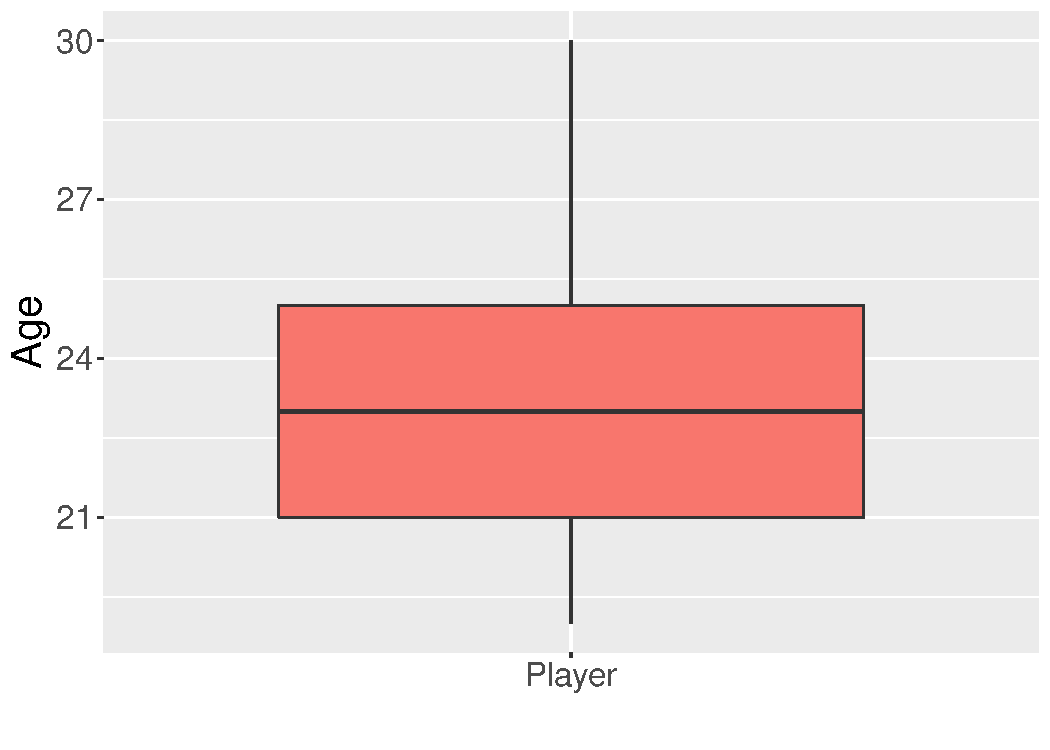
\includegraphics[width=\textwidth]{./appendices/age}
	\caption{Boxplot des Alters der Studienteilnehmer}
	\label{fig:age}
\end{figure}
\todoAll{Alter beschreiben}

\begin{figure}
	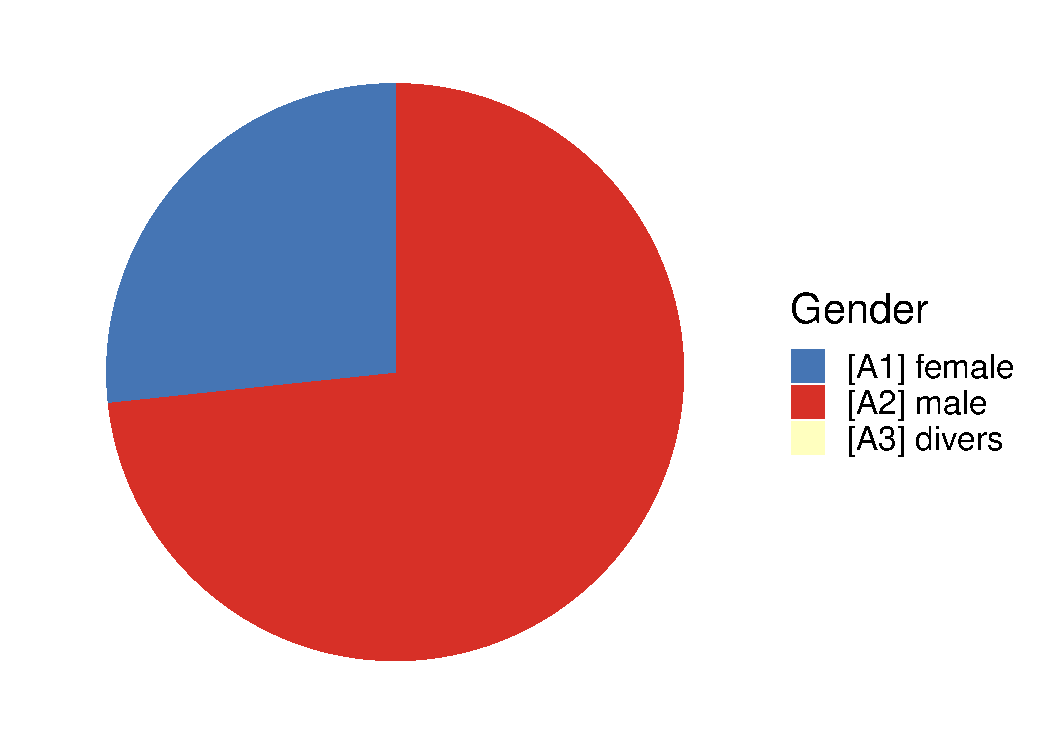
\includegraphics[width=\textwidth]{./appendices/gender}
	\caption{Geschlechterverteilung der Studienteilnehmer}
	\label{fig:gender}
\end{figure}
\todoAll{Geschlecht beschreiben}

\begin{figure}
	% \centering
	\begin{subfigure}{0.48\textwidth}
		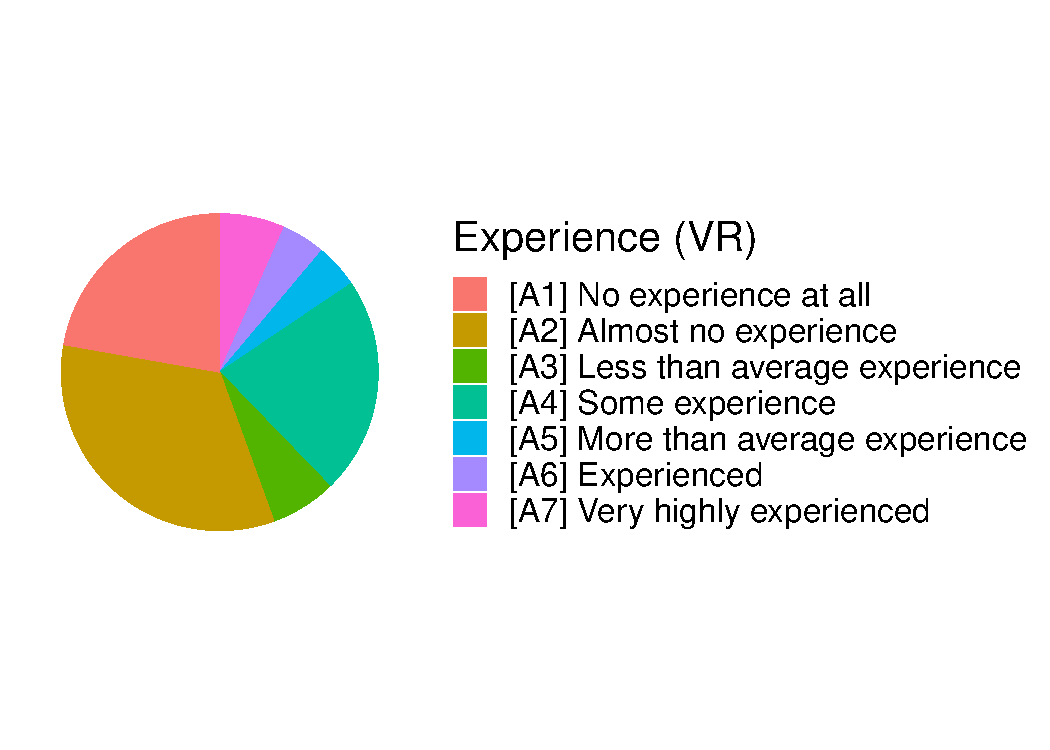
\includegraphics[width=\textwidth]{./appendices/expVr}
		\caption{Grafische Repräsentation der Antworten zur Frage 'How much experience do you have with VR?'.}
		\label{fig:expVr}
	\end{subfigure}%
	\hfill
	\begin{subfigure}{0.48\textwidth}
		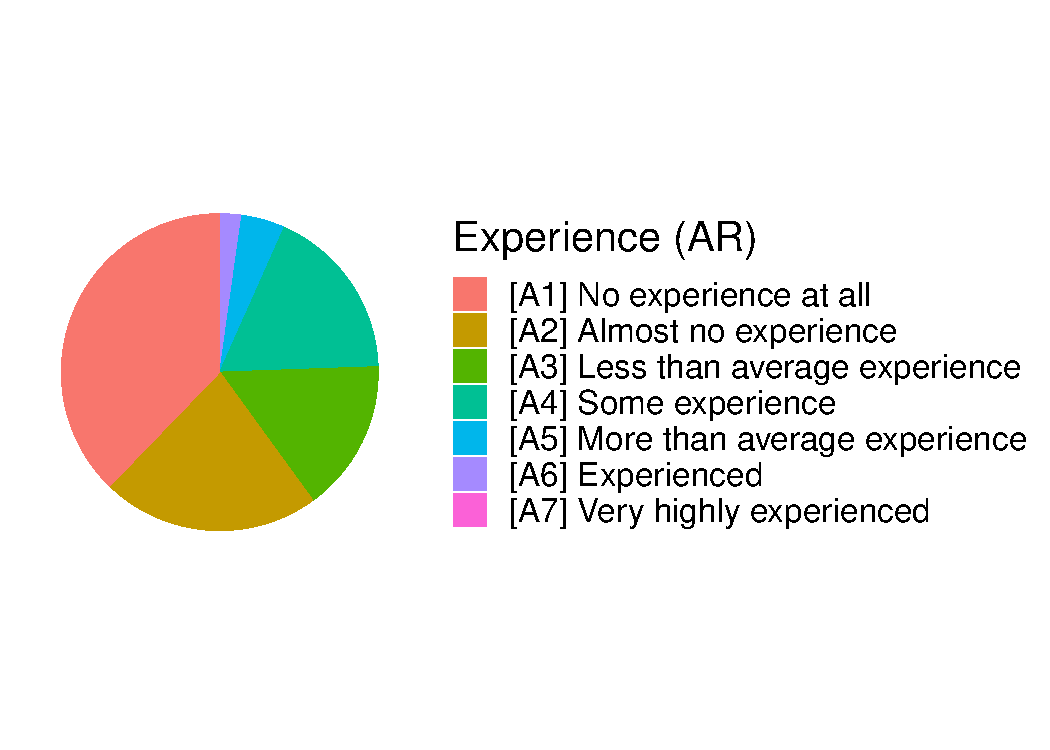
\includegraphics[width=\textwidth]{./appendices/expAr}
		\caption{Grafische Repräsentation der Antworten zur Frage 'How much experience do you have with AR?'.}
		\label{fig:expAr}
	\end{subfigure}
	\caption{Erfahrungen mit virtueller und augmentierter Realität der Studienteilnehmer} % caption for whole figure
\end{figure}
\todoAll{VR/AR Erfahrung beschreiben}

\todoTob{Mehr Ergebnisse einfügen}
\todoAll{Ergebnisse (wertungsfrei) beschreiben}

\begin{figure}
	% \centering
	\begin{subfigure}{0.48\textwidth}
		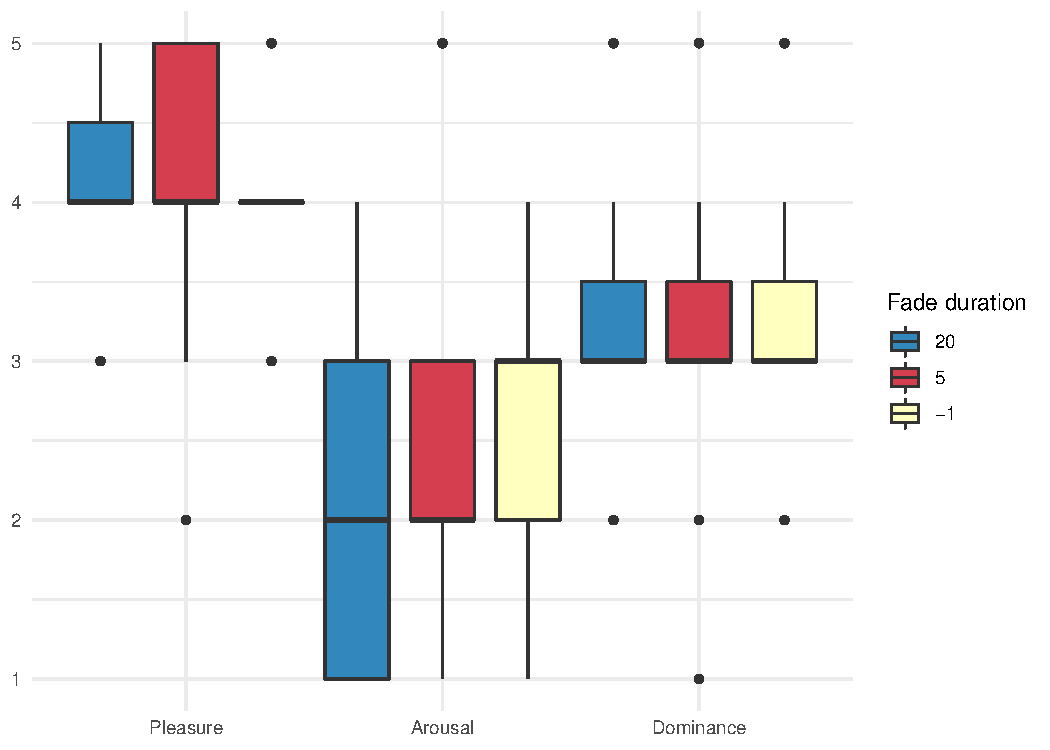
\includegraphics[width=\textwidth]{./appendices/SAMpre}
		\caption{Self-Assessment Manikin Ergebnisse vor der `Schlafphase'}
		\label{fig:samPre}
	\end{subfigure}%
	\hfill
	\begin{subfigure}{0.48\textwidth}
		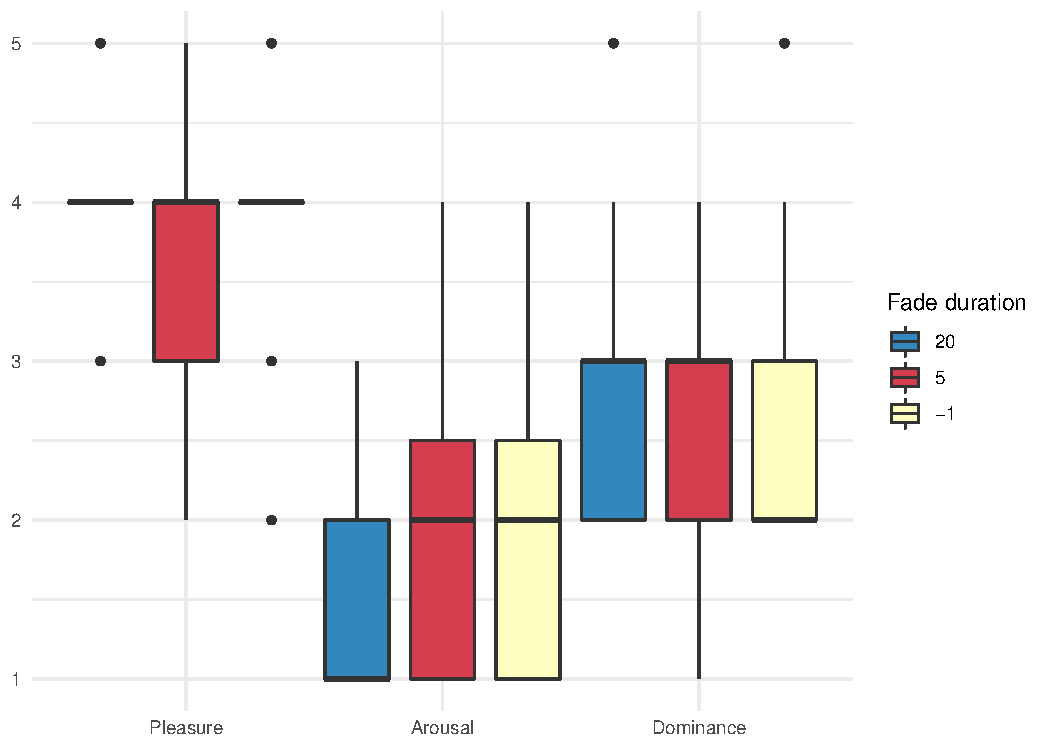
\includegraphics[width=\textwidth]{./appendices/SAMpost}
		\caption{Self-Assessment Manikin Ergebnisse nach der `Schlafphase'}
		\label{fig:samPost}
	\end{subfigure}
	\caption{Die Ergebnisse der Selbsteinschätzung zum Self-Assessment Manikin} % caption for whole figure
\end{figure}
\todoAll{Wie ist das wording für die Schlafphase?? -> ändern}
